\section{Results}
\label{sec:results}

\subsection{Do the gross fuel and flight accounts agree?}

OCAC commercial JP-1 corresponds to 1940.9 kt \COtwo{} in FY2022--23 and 2032.1 kt in
FY2023--24. These values are respectively 0.16\% and 0.77\% below OECD's combined domestic and
international territory estimates (Table~\ref{tab:two-year}). Agreement in the latest two
years is therefore close at the gross commercial boundary.

\begin{table*}[htbp]
\centering
\footnotesize
\begin{tabular}{@{}lrrrrrrrr@{}}
\toprule
 & \multicolumn{4}{c}{\textbf{FY2022--23}} & \multicolumn{4}{c}{\textbf{FY2023--24}} \\
\cmidrule(lr){2-5}\cmidrule(lr){6-9}
\textbf{Component} & \textbf{OCAC kt fuel} & \textbf{OCAC kt \COtwo{}} & \textbf{OECD kt \COtwo{}} & \textbf{Ratio} &
\textbf{OCAC kt fuel} & \textbf{OCAC kt \COtwo{}} & \textbf{OECD kt \COtwo{}} & \textbf{Ratio} \\
\midrule
Resident carriers & 346.0 & 1093.3 & 841.8 & 1.299 & 359.9 & 1137.4 & 884.3 & 1.286 \\
Foreign carriers & 268.2 & 847.6 & 1102.3 & 0.769 & 283.1 & 894.7 & 1163.5 & 0.769 \\
Combined commercial & 614.2 & 1940.9 & 1944.0 & 0.998 & 643.1 & 2032.1 & 2047.8 & 0.992 \\
\bottomrule
\end{tabular}
\caption{Matched carrier-component comparison. Government fuel is excluded from the
commercial boundary.}
\label{tab:two-year}
\end{table*}

The longer record prevents the two-year result from being treated as universal. Across the
five complete OECD overlaps, the combined OCAC/OECD ratio is 0.908, 0.892, 0.935, 0.998 and
0.992 from FY2019--20 to FY2023--24. The nine-year OCAC series also captures the fall in
commercial JP-1 from 730.7 kt in FY2017--18 to 328.7 kt in FY2020--21 and its subsequent
recovery. Monthly combined MAPE is 7.39\% in FY2022--23 and 6.92\% in FY2023--24. Annual
near-closure is thus reproducible in the latest years, but neither historically invariant nor
the product of twelve identical monthly ratios. Full annual and monthly panels are reported in
the supplement.

\subsection{Does agreement survive component decomposition?}

Here, ``resident customers'' are PIA and other Pakistani-airline fuel purchasers in OCAC,
whereas ``resident carriers'' are Pakistani airlines identified in the OECD flight account.
The foreign comparison follows the equivalent OCAC and OECD groups.

Aggregate agreement does not survive this decomposition. Resident-customer fuel is 29.9\% and 28.6\% above OECD resident-carrier emissions
in FY2022--23 and FY2023--24, whereas foreign-customer fuel is 23.1\% below OECD non-resident
emissions in both years. The opposite differences cancel by 99.4\% and 97.0\%, leaving a small
combined discrepancy (Figure~\ref{fig:offsets}). Monthly resident ratios average 1.301 and
1.288, while foreign ratios average 0.770 and 0.768. The sign of the mismatch therefore
persists across both years and months.

\begin{figure}[htbp]
\centering
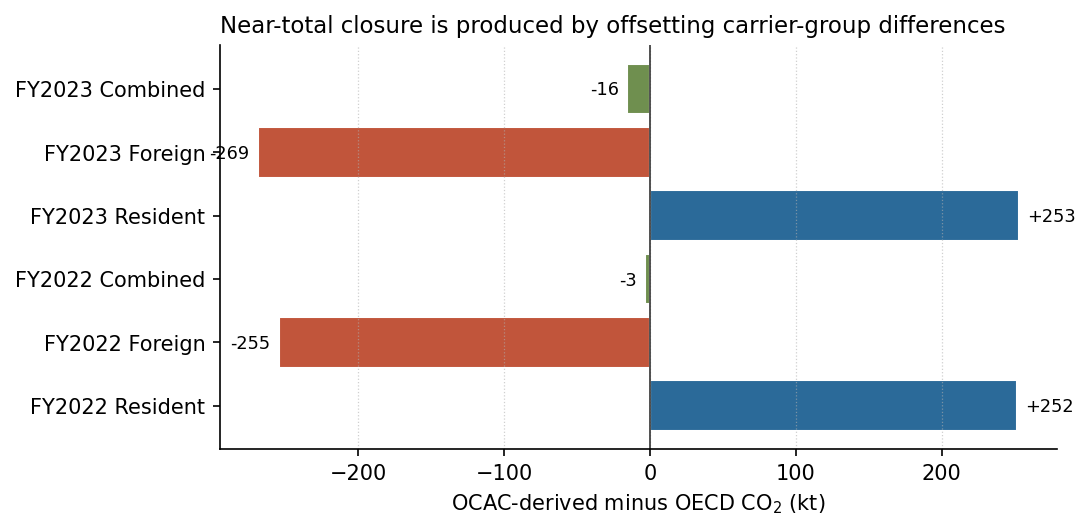
\includegraphics[width=0.92\linewidth]{aviation_component_offsets.png}
\caption{OCAC-derived minus OECD emissions by resident and foreign component. Aggregate
agreement is produced by differences of opposite sign.}
\label{fig:offsets}
\end{figure}

The conserved ledger shows where each reported tonne goes under the central FY2023--24 mapping
(Table~\ref{tab:source-bridge}). PIA and other resident-customer JP-1 contribute 49,760 and
42,649 t to domestic aviation. Their remaining 267,523 t, together with the foreign-customer
row, enters the international-bunker candidate. Government and 100LL streams retain separate
destinations, and an explicit \SI{12282}{\tonne} residual remains unresolved. Every row closes
without using that residual to improve the apparent agreement.

\begin{table*}[htbp]
\centering
\footnotesize
\begin{tabular}{@{}lrrrrrr@{}}
\toprule
\textbf{OCAC source row} & \textbf{Reported t} & \textbf{Domestic} & \textbf{Bunker} &
\textbf{Military} & \textbf{General aviation} & \textbf{Residual} \\
\midrule
Domestic Avi--PIA, JP-1 & 193,813 & 49,760 & 144,053 & --- & --- & --- \\
Domestic Avi--Others, JP-1 & 166,119 & 42,649 & 123,470 & --- & --- & --- \\
Overseas/Foreign Aviation, JP-1 & 283,147 & --- & 283,147 & --- & --- & --- \\
Government Aviation, JP-1 & 2,973 & --- & --- & 2,973 & --- & --- \\
Government Other, JP-1 & 12,282 & --- & --- & --- & --- & 12,282 \\
Government Other, JP-8 & 117,785 & --- & --- & 117,785 & --- & --- \\
All reported 100LL & 4,542 & --- & --- & --- & 4,542 & --- \\
\midrule
\textbf{Total} & \textbf{780,661} & \textbf{92,409} & \textbf{550,670} &
\textbf{120,758} & \textbf{4,542} & \textbf{12,282} \\
\bottomrule
\end{tabular}
\caption{FY2023--24 source-row-conserving fuel bridge under the OECD-calibrated resident
share. Dashes denote zero assignments.}
\label{tab:source-bridge}
\end{table*}

Because customer classes cannot directly supply the domestic boundary, we next compare
alternative estimates of domestic aviation.

\subsection{What does the bridge imply for domestic aviation?}

Using OECD's resident-carrier domestic share assigns 92,409 t of fuel, or 292.0 kt \COtwo{},
to domestic aviation (Table~\ref{tab:bridge-results}). The aggregate movement estimate is
298.9 kt, only 2.3\% higher. Because OECD supplies the partition, this agreement is a
consistency check. Against the independent OECD domestic-territory value of
235.8 kt, the aggregate movement model is 26.8\% higher, the route-resolved model is 14.8\%
higher and the completed route--aircraft model (M2) is 4.7\% higher.

\begin{table}[htbp]
\centering
\scriptsize
\begin{tabular}{@{}lrrr@{}}
\toprule
\textbf{Estimate} & \textbf{Fuel (t)} & \textbf{kt \COtwo{}} & \textbf{Role} \\
\midrule
Aggregate movement (M0) & 94,576 & 298.9 & Unconstrained \\
Route-resolved (M1) & 85,669 & 270.7 & Unconstrained \\
Calibrated fuel bridge & 92,409 & 292.0 & OECD-calibrated \\
Movement-share bridge & 107,555 & 339.9 & Structural \\
Literal customer labels & 359,932 & 1137.4 & Diagnostic \\
Completed route--aircraft model (M2) & 78,139 & 246.9 & Provisional \\
OECD domestic territory & --- & 235.8 & External \\
\bottomrule
\end{tabular}
\caption{FY2023--24 domestic \COtwo{} estimates. Different evidence roles preclude averaging
the rows into one preferred value.}
\label{tab:bridge-results}
\end{table}

The same ordering broadly replicates in FY2022--23: aggregate movement fuel is 101,196 t,
route-resolved fuel 90,446 t, the calibrated bridge 94,314 t and OECD domestic territory
237.2 kt \COtwo{}. Including CH4 and N2O gives
\SI{0.294}{\mega\tonne} \COe{} for the FY2023--24 bridge, compared with 0.301 Mt for the
aggregate movement model. The central bridge also assigns 550,670 t of commercial JP-1 to
full-flight international bunkers, or \SI{1.740}{\mega\tonne} \COtwo{}. That quantity is
distinct from the 210.4 kt international LTO estimate at Pakistani airports. The
non-commercial fuel the bridge identifies is now priced too, as memo rows beside the
bunkers: 120,758~t of military and government jet fuel (\SI{381.6}{\giga\gram}
\COtwo{}), 4,542~t of 100LL general aviation (\SI{14.1}{\giga\gram}) and 12,282~t of
unresolved government JP-1 (\SI{38.8}{\giga\gram})---together about
\SI{0.434}{\mega\tonne}, larger than the reported domestic sector, outside the
1.A.3.a total because IPCC books military aviation under 1A5b and no record attributes
the activity; the scope choice is priced against the national total as three
independent configurations, one per fuel evidence class, and the same
streams ship as a first-class OBSERVED-UNALLOCATED ACCOUNT
(\texttt{outputs/aviation\_unallocated\_fuel\_fy2023\_24.csv}: each identified tonne
with a closed evidence class, its disposition, and the record that would close
it), so booked-outside-the-boundary can never read as absent, because military
attribution, general-aviation activity and the bridge residual are separate
questions: \emph{military\_government\_in\_scope} (\num{445.33702}~Mt),
\emph{general\_aviation\_in\_scope} (\num{444.96950}~Mt) and
\emph{unresolved\_jp1\_in\_scope} (\num{444.99423}~Mt), each against the
\num{444.95542} reference.

\begin{figure}[htbp]
\centering
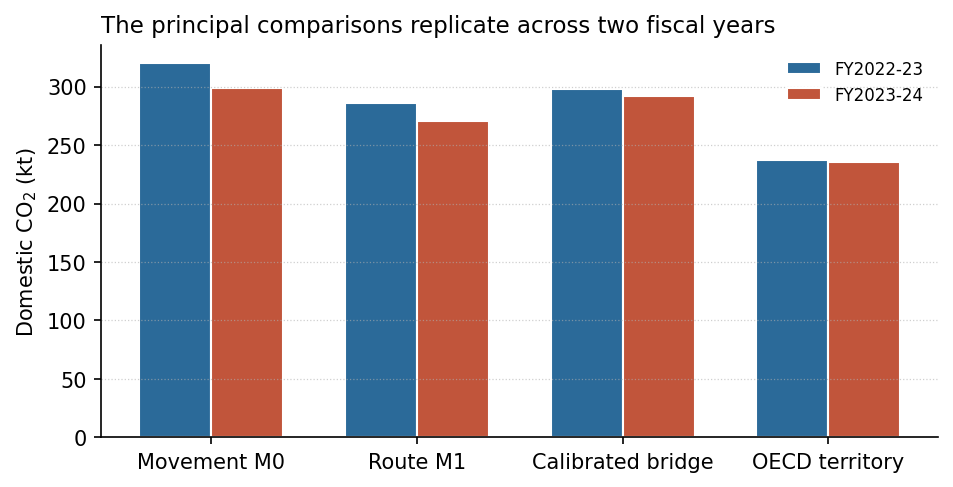
\includegraphics[width=\linewidth]{aviation_two_year.png}
\caption{Two-year comparison of aggregate movement, route-resolved, calibrated-bridge and
OECD domestic estimates.}
\label{fig:domestic-comparison}
\end{figure}

\begin{figure*}[htbp]
\centering
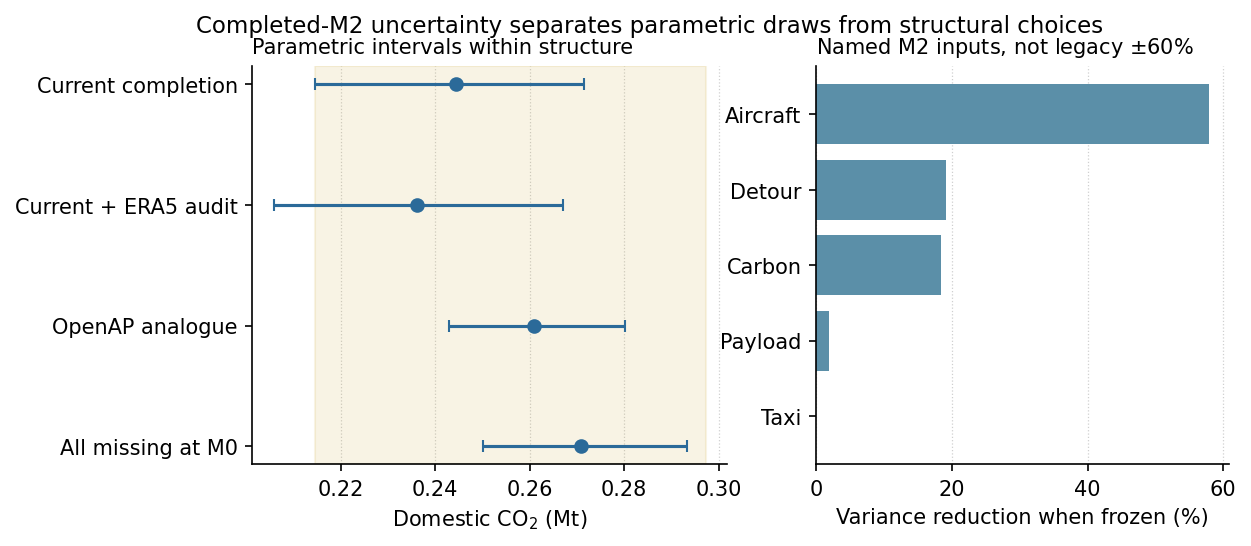
\includegraphics[width=0.78\textwidth]{aviation_m2_uncertainty.png}
\caption{Route--aircraft Monte Carlo intervals, structural envelope and drop-one variance
diagnostics for the completed route--aircraft model.}
\label{fig:route-aircraft-uncertainty}
\end{figure*}

Carrier-specific scenarios change attribution within the resident rows but not the calibrated
total. After constraining separate PIA and other-carrier movement shares to the same aggregate,
their domestic shares are 20.0\% and 32.2\%. Partial modelled-fuel shares are not used because
only 27.9\% of resident international departures are reconstructed.

\subsection{Are the findings supported by other evidence?}

Pakistan's official calendar-2022 CRT reports 654.1 kt domestic and 163.5 kt international
aviation \COtwo{}, compared with matched OECD values of 232.9 and 1713.3 kt
(Figure~\ref{fig:official}a). The official workbook applies an explicit 80\% domestic and 20\%
international fuel distribution, labels the activity aviation gasoline and marks jet kerosene
not estimated. Its domestic and international ratios to OECD are therefore 2.808 and 0.095.
The reported allocation is not consistent with the petroleum and flight-geography evidence
examined here, and its institutional derivation could not be reconstructed. The supplement
provides the workbook hash and cell-level audit.

Climate TRACE gives 255.9 kt domestic and 1950.9 kt international \COtwo{} for FY2023--24,
8.5\% and 7.7\% above OECD. Its airport ordering is strongly associated with PCAA activity:
Spearman's $\rho=0.971$ across 16 domestic airports and 0.948 across 11 international airports
(Figure~\ref{fig:official}b). This supports the broad spatial pattern, not independent fuel-burn
accuracy.

\begin{figure*}[htbp]
\centering
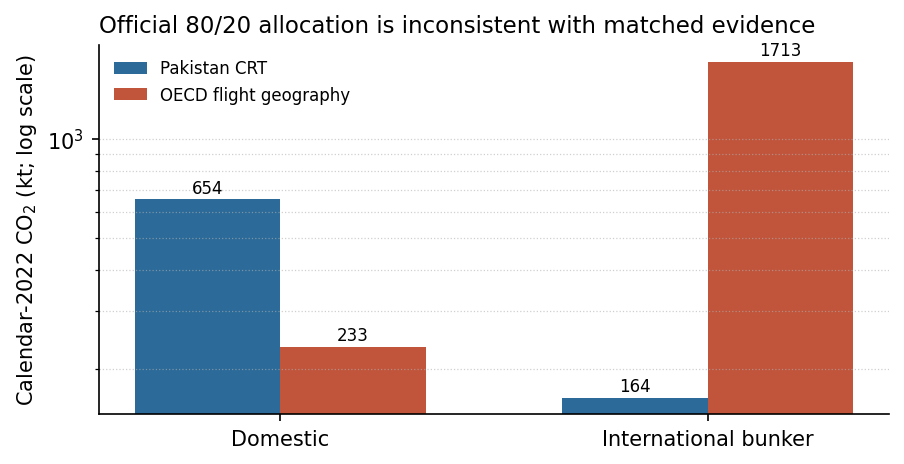
\includegraphics[width=0.43\textwidth]{aviation_official_reporting.png}\hfill
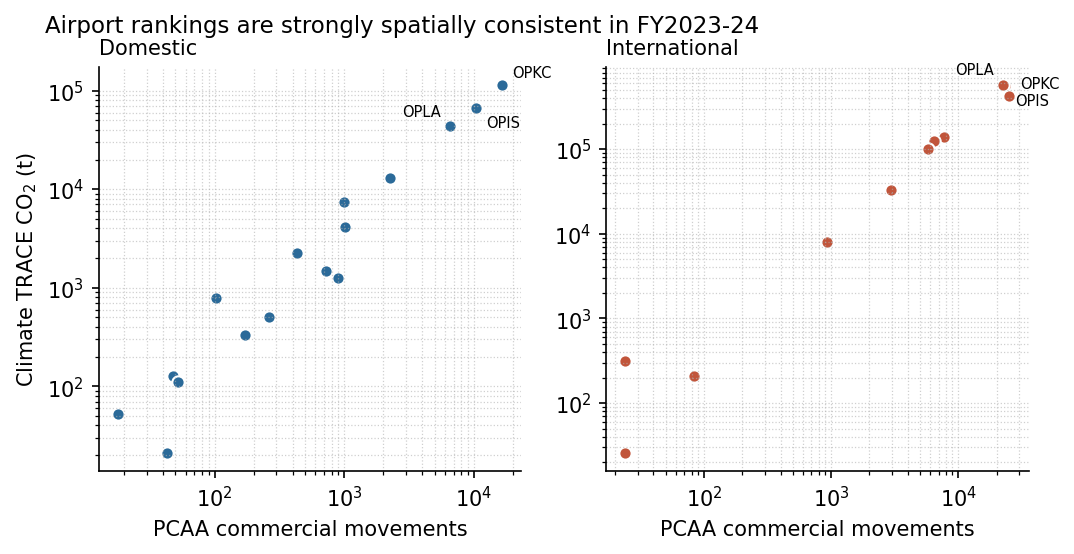
\includegraphics[width=0.54\textwidth]{aviation_climatetrace_airports.png}
\caption{External diagnostics. (a) Pakistan's calendar-2022 CRT categories versus matched
OECD flight-geography estimates. (b) FY2023--24 PCAA airport movements versus Climate TRACE
airport \COtwo{}.}
\label{fig:official}
\end{figure*}

\subsection{What remains uncertain?}

The documented route graph allocates 20,098 of 20,300 domestic stages. Conditional on PCAA
margins and supported links, its minimum, central and maximum mean distances are 485.2, 486.5
and 503.0 nmi. On identical 17,491-stage support, aggregate factors produce 81,490 t fuel,
route-specific distance 76,102 t and route--aircraft profiles 73,439 t. Route resolution lowers
fuel by 6.6\% and the aircraft/performance layer by a further 3.5\%. Explicit completion of
unsupported aircraft and unallocated activity yields 78,139 t.

For the central structure, the route--aircraft Monte Carlo gives mean domestic emissions of
0.244 Mt \COtwo{} from 20,000 draws
(95\% interval 0.215--0.272 Mt). Alternative route graphs and completion methods widen the
endpoint envelope to 0.215--0.297 Mt. Aircraft assignment reduces simulated variance by
57.9\% when frozen, followed by detour (19.2\%) and carbon conversion (18.4\%); these drop-one
responses are non-additive. The remaining uncertainty is consequently tied to identifiable
flight-stage quantities rather than the aggregate model's umbrella representation term.

Supplementary tests support the treatment of the completed route--aircraft model. A physical
range assertion identified and corrected an OpenAP distance-unit mismatch, after which the
common-support performance difference fell from 39.4\% to 3.5\%. Sampled ERA5 winds changed
representative fuel by $-3.9$\% on average. A four-day ADSB.lol pilot provided no usable
Pakistan-airport stages despite passing synthetic and same-archive positive controls;
reconstructed activity is therefore retained rather than expanded from inadequate
observations.
